\documentclass{beamer}
\usepackage[portuguese]{babel}
\usetheme{uic}
\usepackage{amsfonts,amsmath,oldgerm,algorithmic,algorithm}
\usepackage[font=small,labelfont=bf]{caption} % Required for specifying captions to tables and figures

\newcommand{\hrefcol}[2]{\textcolor{uihteal}{\href{#1}{#2}}}
\newcommand{\testcolor}[1]{\colorbox{#1}{\textcolor{#1}{test}}~\texttt{#1}}

% Please see Section 18.1 of Beamer User Guide for all the options \usefonttheme provides
\usefonttheme[onlymath]{serif}
% \usefonttheme{serif} % use this if you would like Serif font throughout (and not just for math)

\title{MODELO FRACTAL DE UMA DESCARGA COMPACTA INTRA-NUVEM. I. CARACTERÍSTICAS DA ESTRUTURA E EVOLUÇÃO.}
\titlebackground{images/tema_fundo_2.png}
% an asterisk will split the background:
% \titlebackground*{images/uic_seo.jpg}
\subtitle{D. I. Iudin and S. S. Davydenko, 2015}

\author{\href{mailto:augusto.adamns@ufpr.br}{Augusto Mathias Adams}}
\date{\today}

\begin{document}
\themecolor{maintitle}
\maketitle
\themecolor{light}
% default is no footline, but page numbers are incredibly useful for the audience to ask questions later
\footlinecolor{uicblue}

\begin{frame}{Introdução}
	\begin{itemize}
		\item Novo modelo de descargas compactas intra-nuvem (\textbf{\textit{CID}}), que se baseia na abordagem fractal para a descrição de sua estrutura elétrica.
		\item 2 etapas:
		\begin{itemize}
			\item Desenvolvimento de \textit{streamers}
			\item Conexão entre os \textit{streamers}
		\end{itemize}
		\item Sincronização espacial e temporal das estruturas
	\end{itemize}
\end{frame}

\begin{frame}{Introdução}
	\begin{itemize}
		\item \textit{\textbf{\alert{Motivação $\Rightarrow$}}} Restrições dos modelos anteriores:
		\begin{itemize}
			\item Falta de crescimento simultâneo de ramos da descarga
			\item Ausência de consideração das correntes
		\end{itemize}
		\item Baseado em autômatos celulares
		\item Ligações elétricas entre células através de descargas elétricas
		\item Modelo que contempla apenas uma parte do volume do meio intra-nuvem
	\end{itemize}
\end{frame}

\begin{chapter}[images/tema_fundo_5.png]{uicblue}{Modelo Fractal}
\textit{Modelagem em Etapas}
\end{chapter}

\begin{frame}{\textit{Streamer}}
	\begin{columns}
		\begin{column}{0.5\textwidth}
			\begin{figure}
				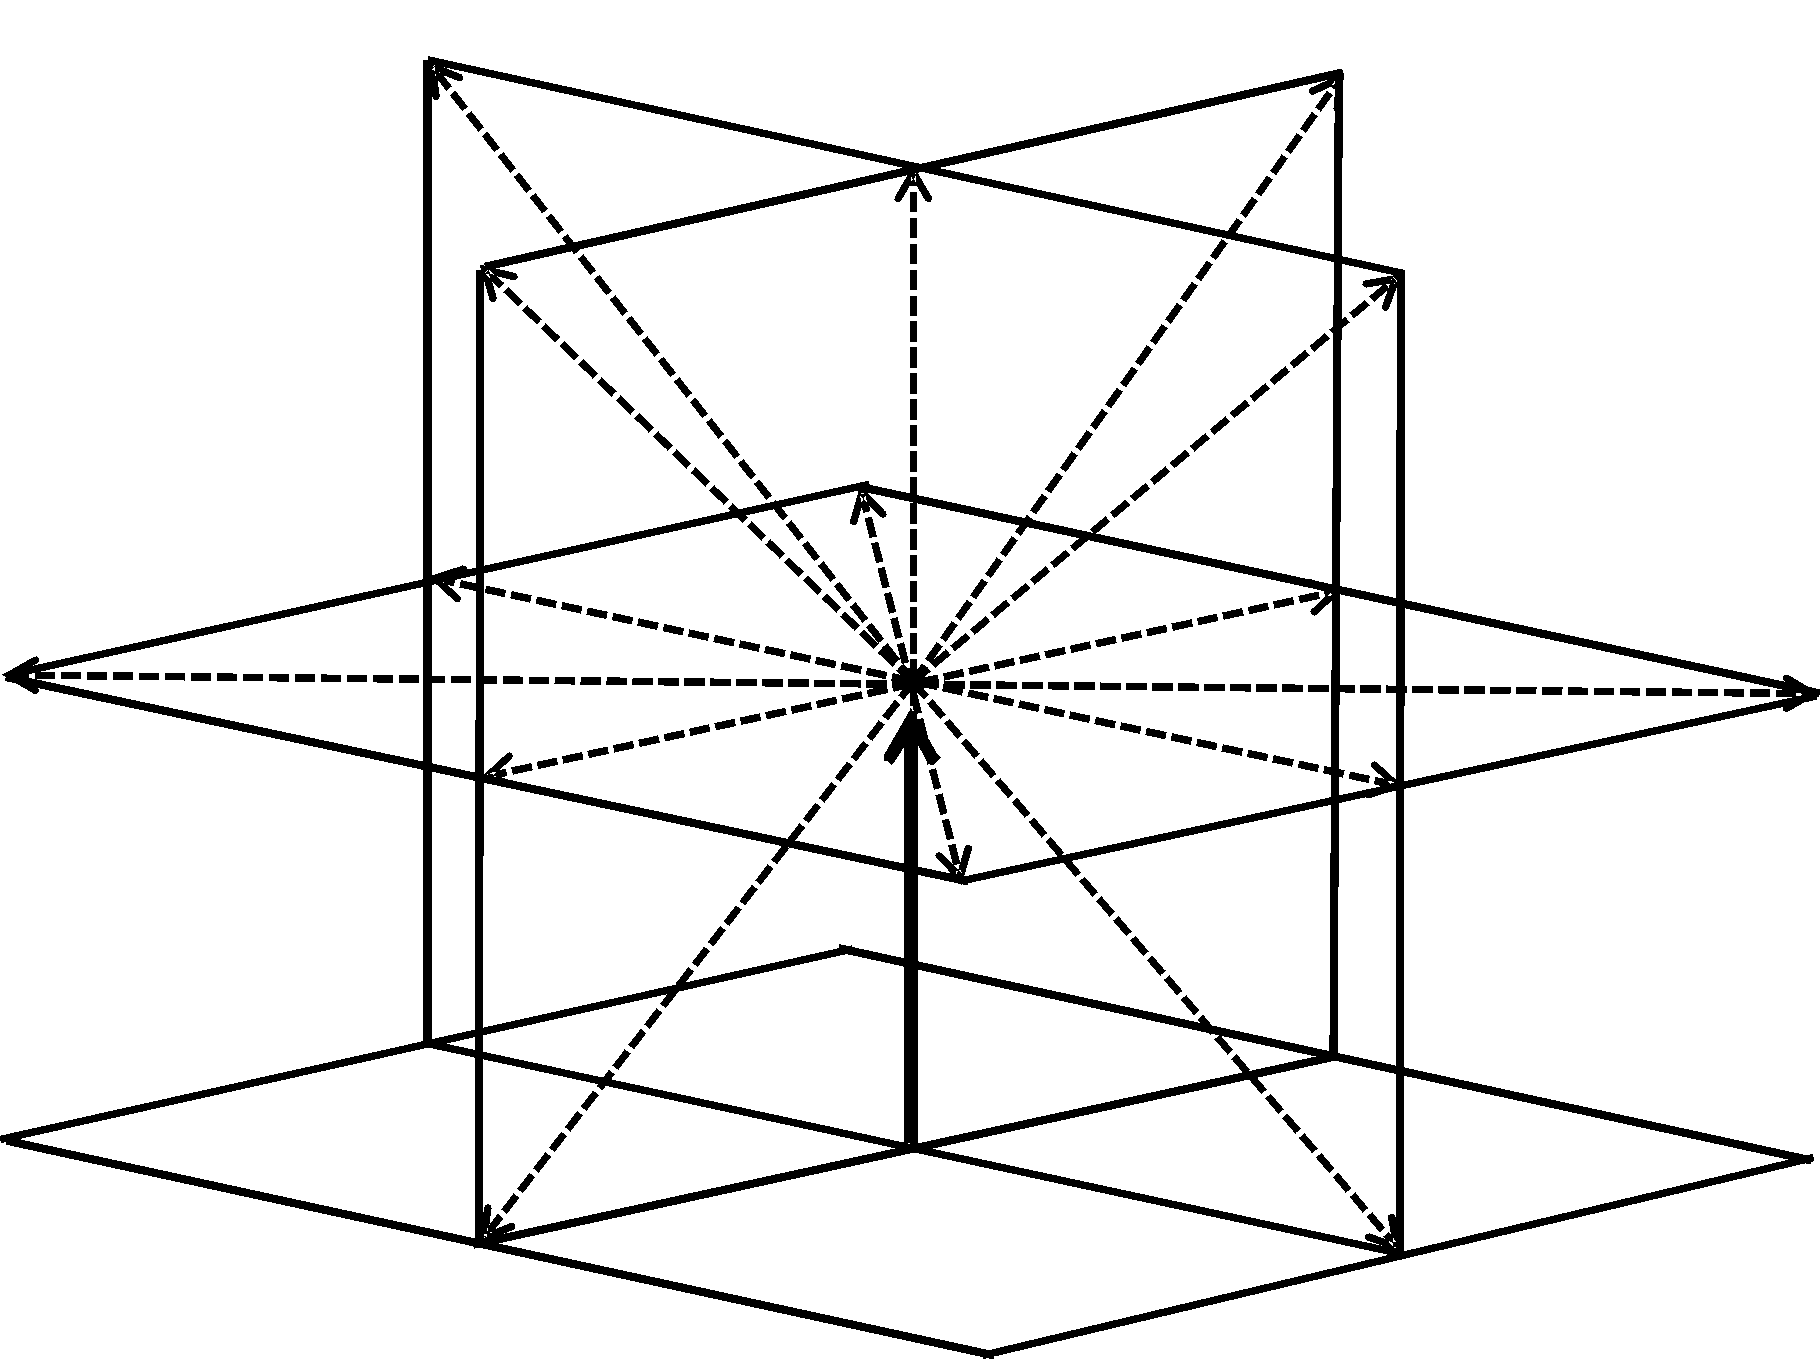
\includegraphics[height=0.6\textheight]{imagens_artigo/5.png}
				\captionof{figure}{Autômato Celular}
			\end{figure}
		\end{column}
		\begin{column}{0.5\textwidth}
			\begin{itemize}
				\item Região espacial: $500m \times 500 m\times 500 m$
				\item Autômatos: células de $10m \times 10m \times 10m$
				\begin{itemize}
					\item \textbf{Cada autômato é representado pelo seu centro de massa e sua respectiva carga $q_{ij}$.}
				\end{itemize}
			\end{itemize}
		\end{column}
	\end{columns}
\end{frame}

\begin{frame}{\textit{Streamer}}
	\begin{columns}
		\begin{column}{0.5\textwidth}
			\begin{equation}
				P_{ij} = \begin{cases}
					1 - exp \left( -\left| \frac{E_{ij} - E_i}{E_s - E_i} \right|^m\right ), &  E_{ij} \geq E_i \\ 
					0, & E_{ij} < E_i 
				\end{cases}
				\label{eqn_1}
			\end{equation}
			\begin{equation}
				dq_i = \tau \sum_{j=1}^{a_i + b_i} I_{ij} 
				\label{eqn_2}
			\end{equation}
			\begin{equation}
				I_{ij} = \frac{\phi_i - \phi_j}{\Re_{ij} L_{ij}}
				\label{eqn_3}
			\end{equation}
		\end{column}
		\begin{column}{0.5\textwidth}
			\begin{figure}
				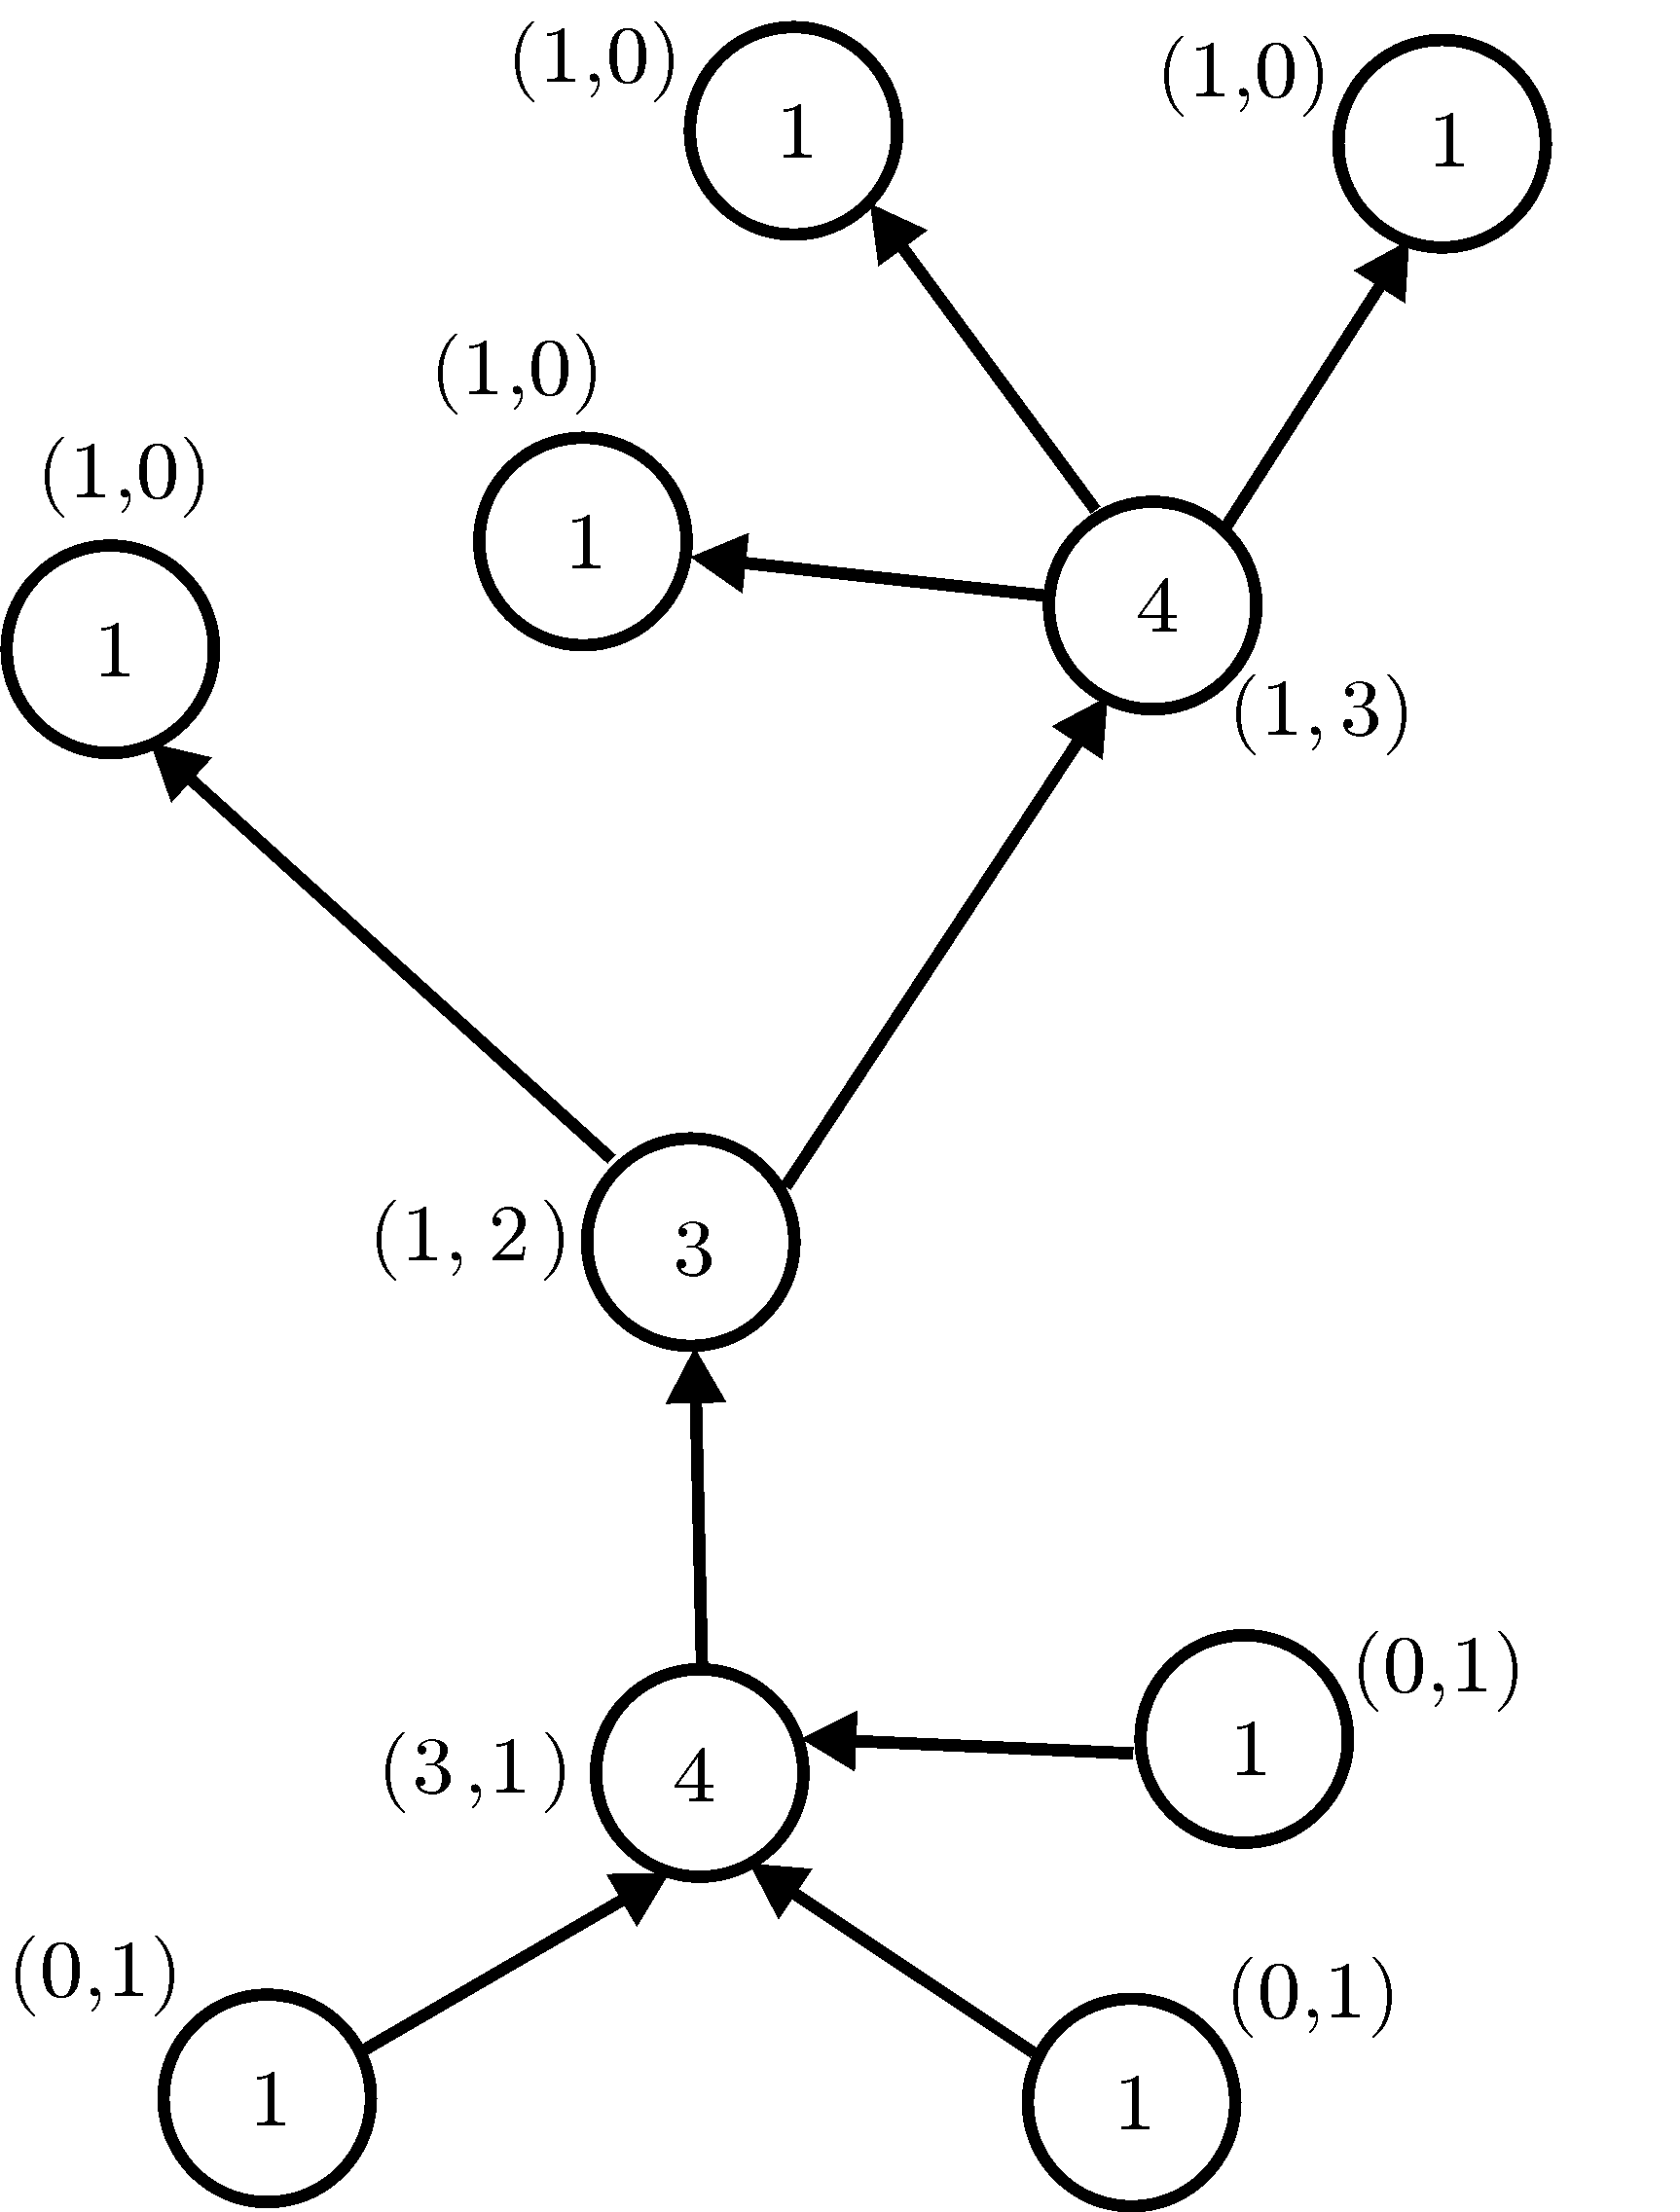
\includegraphics[height=0.8\textheight]{imagens_artigo/6.png}
				\captionof{figure}{Árvore de Descarga}
			\end{figure}
		\end{column}
	\end{columns}
\end{frame}

\begin{frame}{\textit{Streamer}}
	\begin{columns}
		\begin{column}{0.33\textwidth}
			\begin{figure}
				\centering
				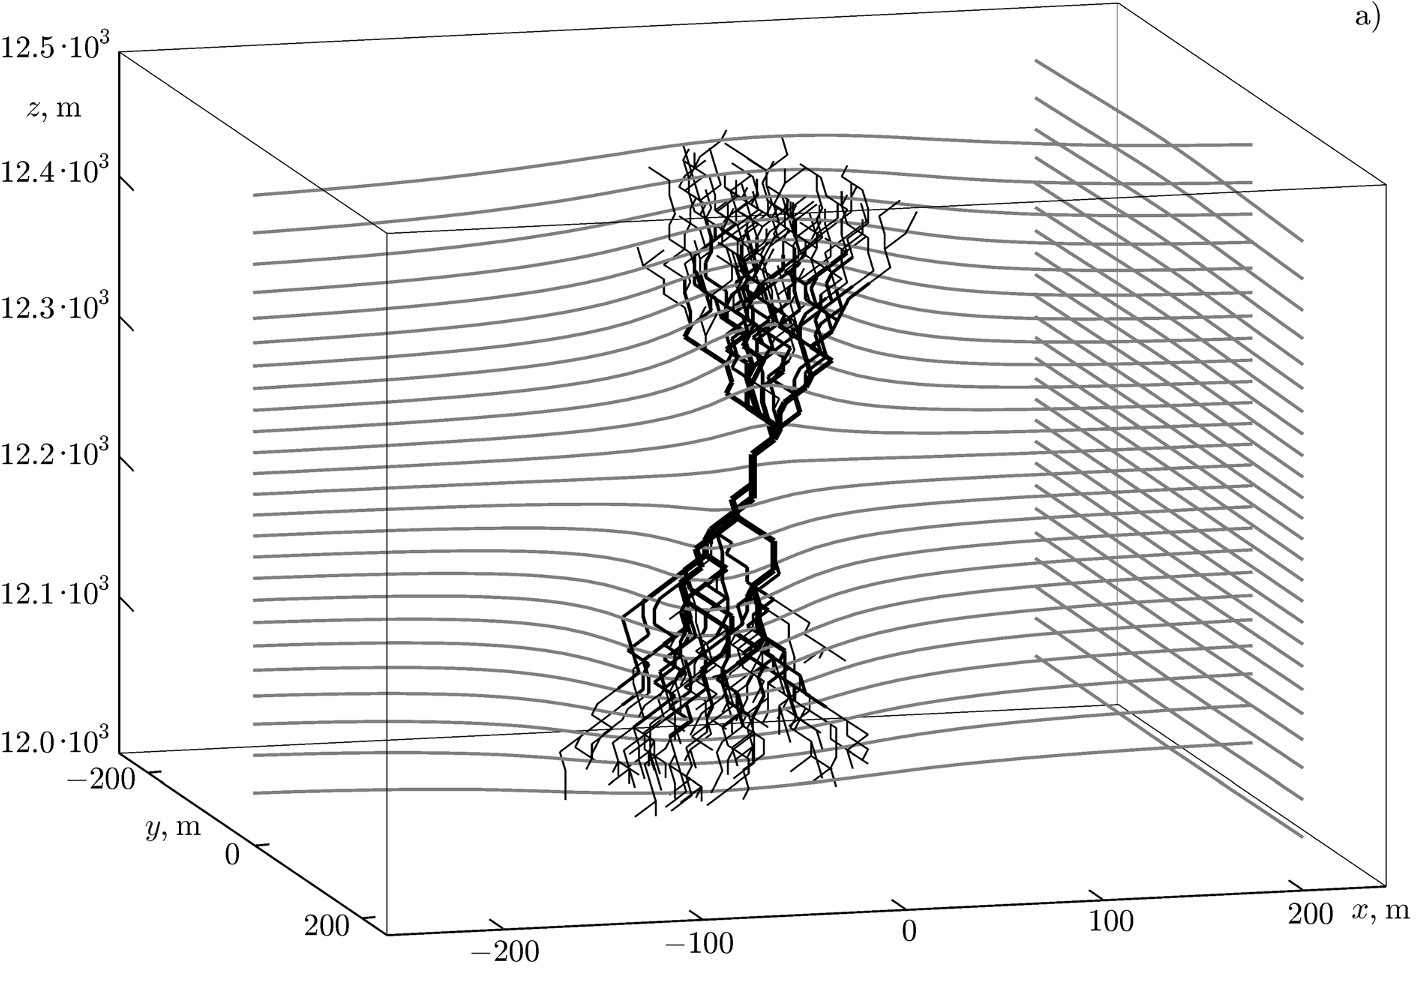
\includegraphics[width=0.9\textwidth]{imagens_artigo/9.png}
				\captionof{figure}{Streamer Desenvolvido}
			\end{figure}
		\end{column}
		\begin{column}{0.67\textwidth}
			\begin{figure}
				\centering
				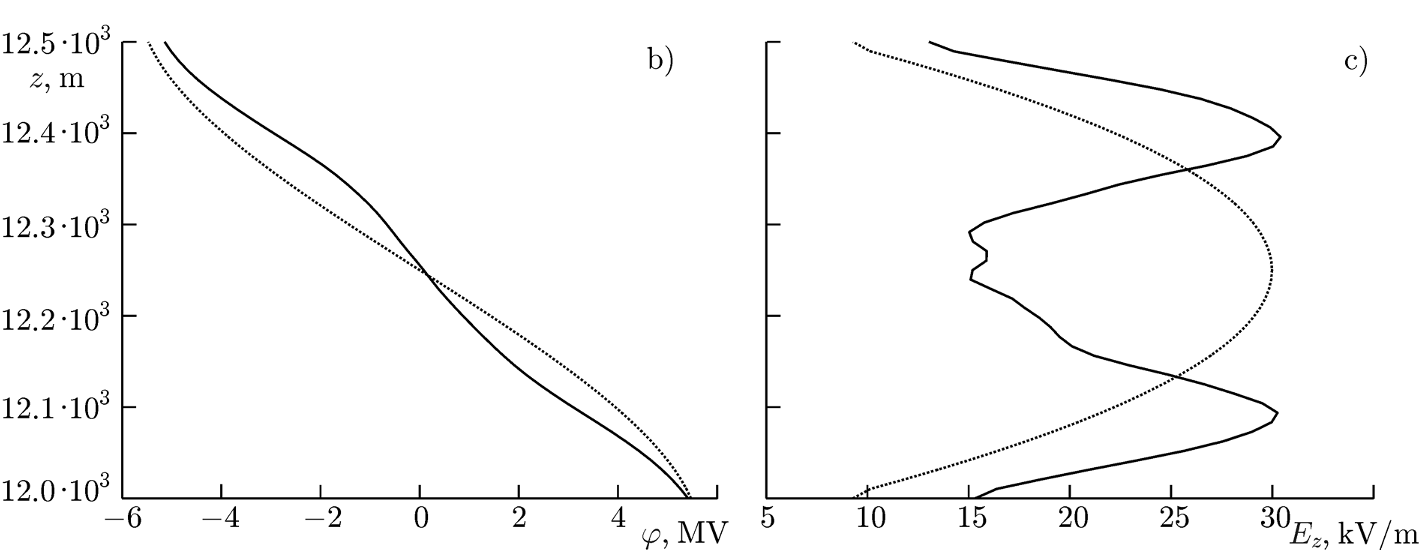
\includegraphics[width=0.9\linewidth]{imagens_artigo/9b}
				\captionof{figure}{Potencial e Campo Elétrico Vertical ao longo da linha de descarga}
				\label{fig:9b}
			\end{figure}
			
		\end{column}
	\end{columns}
\end{frame}

\begin{frame}{Sincronização dos \textit{Streamers}}
	\begin{columns}
		\begin{column}{0.5\textwidth}
			\begin{equation}
				\gamma_{max} = \begin{cases}
					4\pi\sigma\left(\Omega/\vartheta-1\right)^2, & \Omega/\vartheta < 2 \\ 
					2\pi\sigma/\vartheta, & \Omega/\vartheta > 2 
				\end{cases}
				\label{eqn_4}	
			\end{equation}
			\begin{equation}
				k_{opt} = \begin{cases}
					\frac{\vartheta}{u} \left(\frac{\Omega}{\vartheta}-1\right)^{\frac{1}{2}}& \Omega/\vartheta < 2 \\ 
					\sigma/\vartheta, & \Omega/\vartheta > 2 
				\end{cases}
				\label{eqn_5}	
			\end{equation}
		\end{column}
		\begin{column}{0.5\textwidth}
			\begin{itemize}
				\item Iniciação do \textbf{\textit{CID}} pressupõe a formação de duas estruturas de \textit{streamer} bipolar desenvolvidas.
				\item Sincronização espaço-temporal das descargas de \textit{streamer} é importante
				\item Solução possível: desenvolvimento sincronizado de descargas devido à instabilidade do fluxo ascendente.
			\end{itemize}
		\end{column}
	\end{columns}
\end{frame}
\begin{frame}{\textit{Sincronização dos Streamers}}

	\begin{figure}
		\centering
		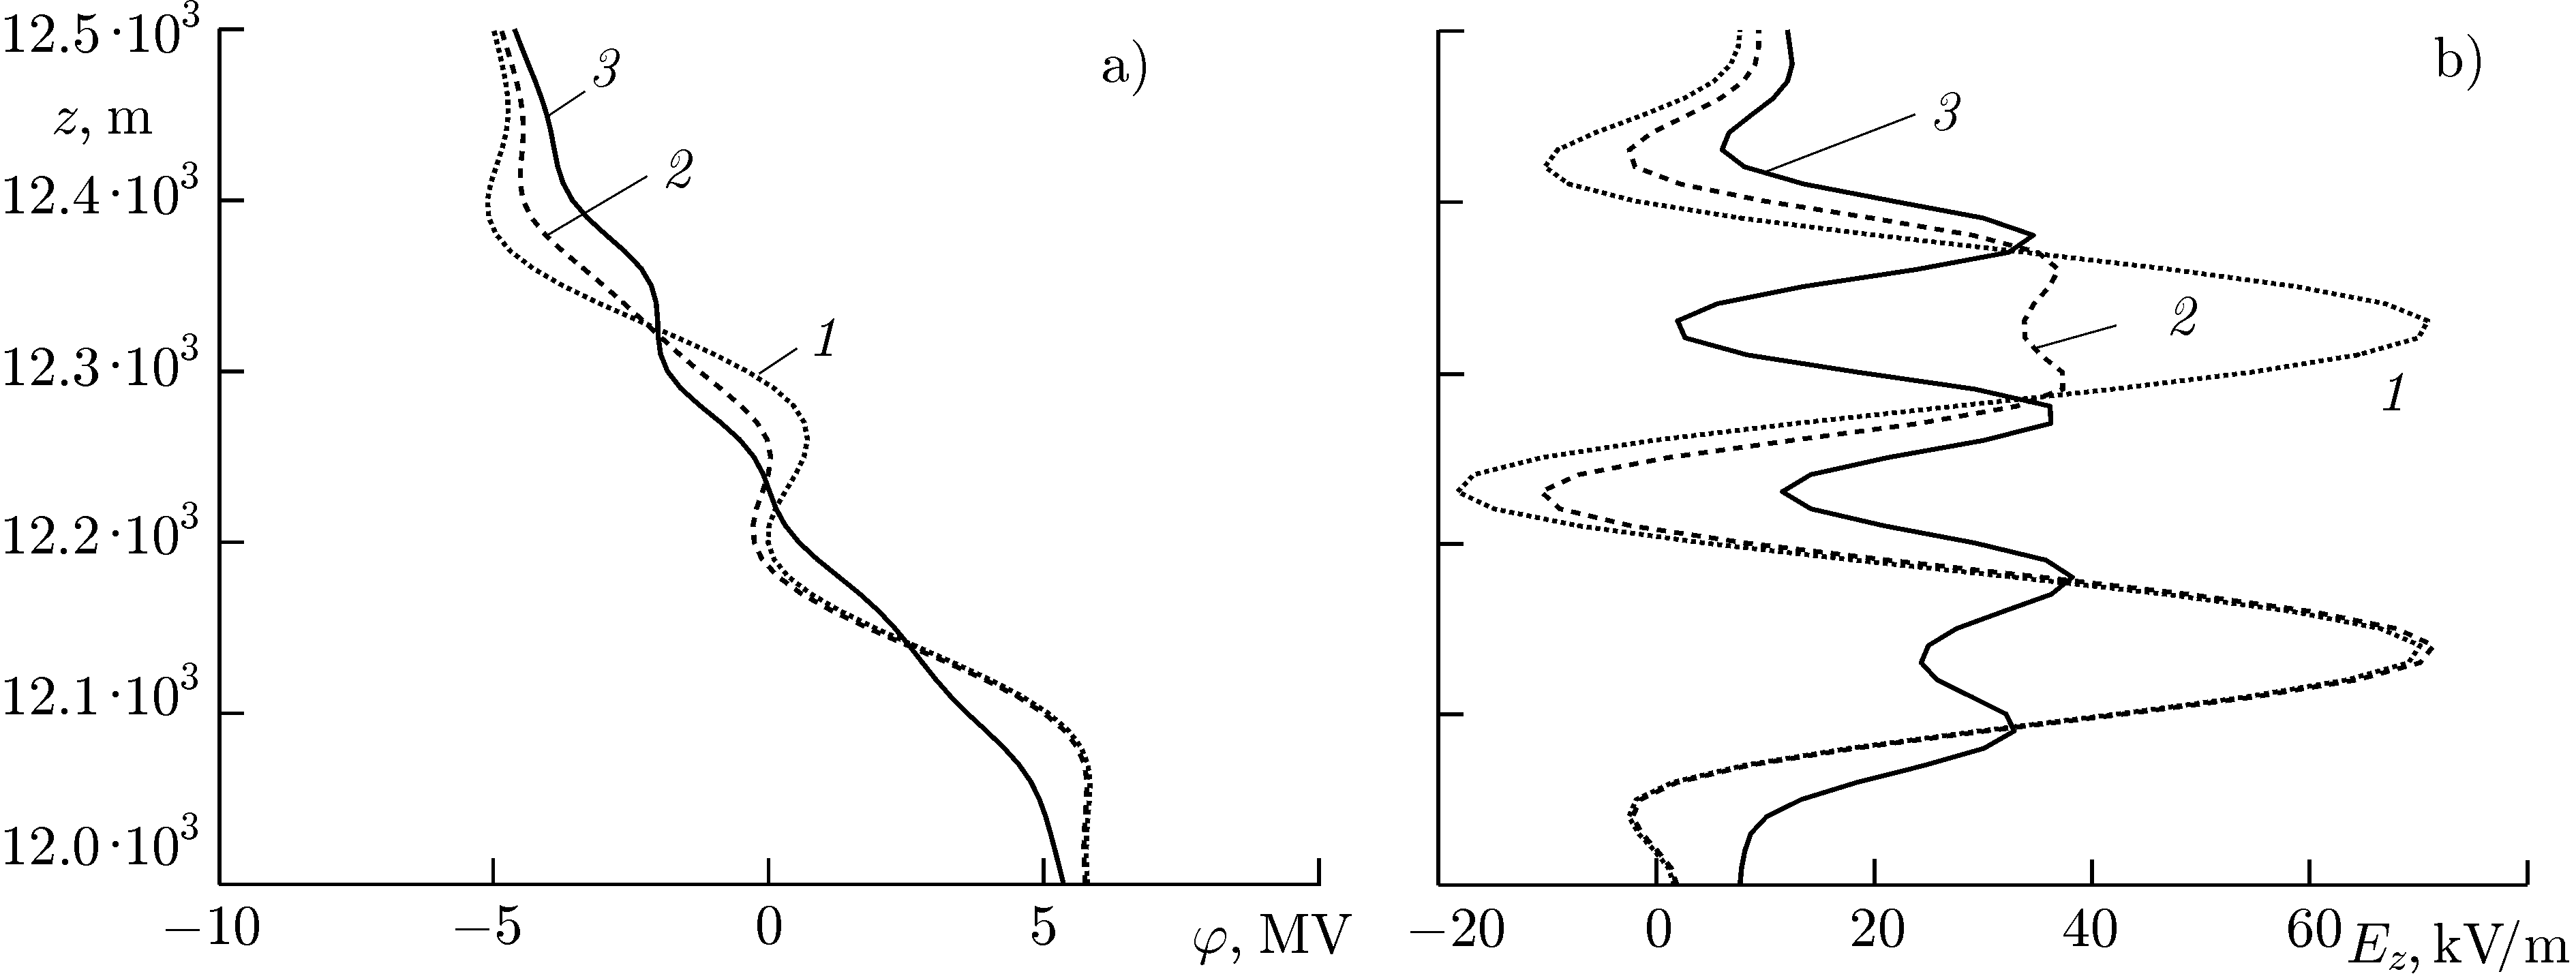
\includegraphics[width=0.9\textwidth]{imagens_artigo/12.png}
		\captionof{figure}{Potencial e Campo Elétrico Vertical ao Longo da Descarga}
	\end{figure}
		
\end{frame}

\begin{chapter}[images/tema_fundo_6.png]{uicblue}{Descarga CID}
\textit{Resultados do Modelo}
\end{chapter}

\begin{frame}{\textit{Resultados}}
	\begin{columns}
		\begin{column}{0.5\textwidth}
			\begin{figure}
				\centering
				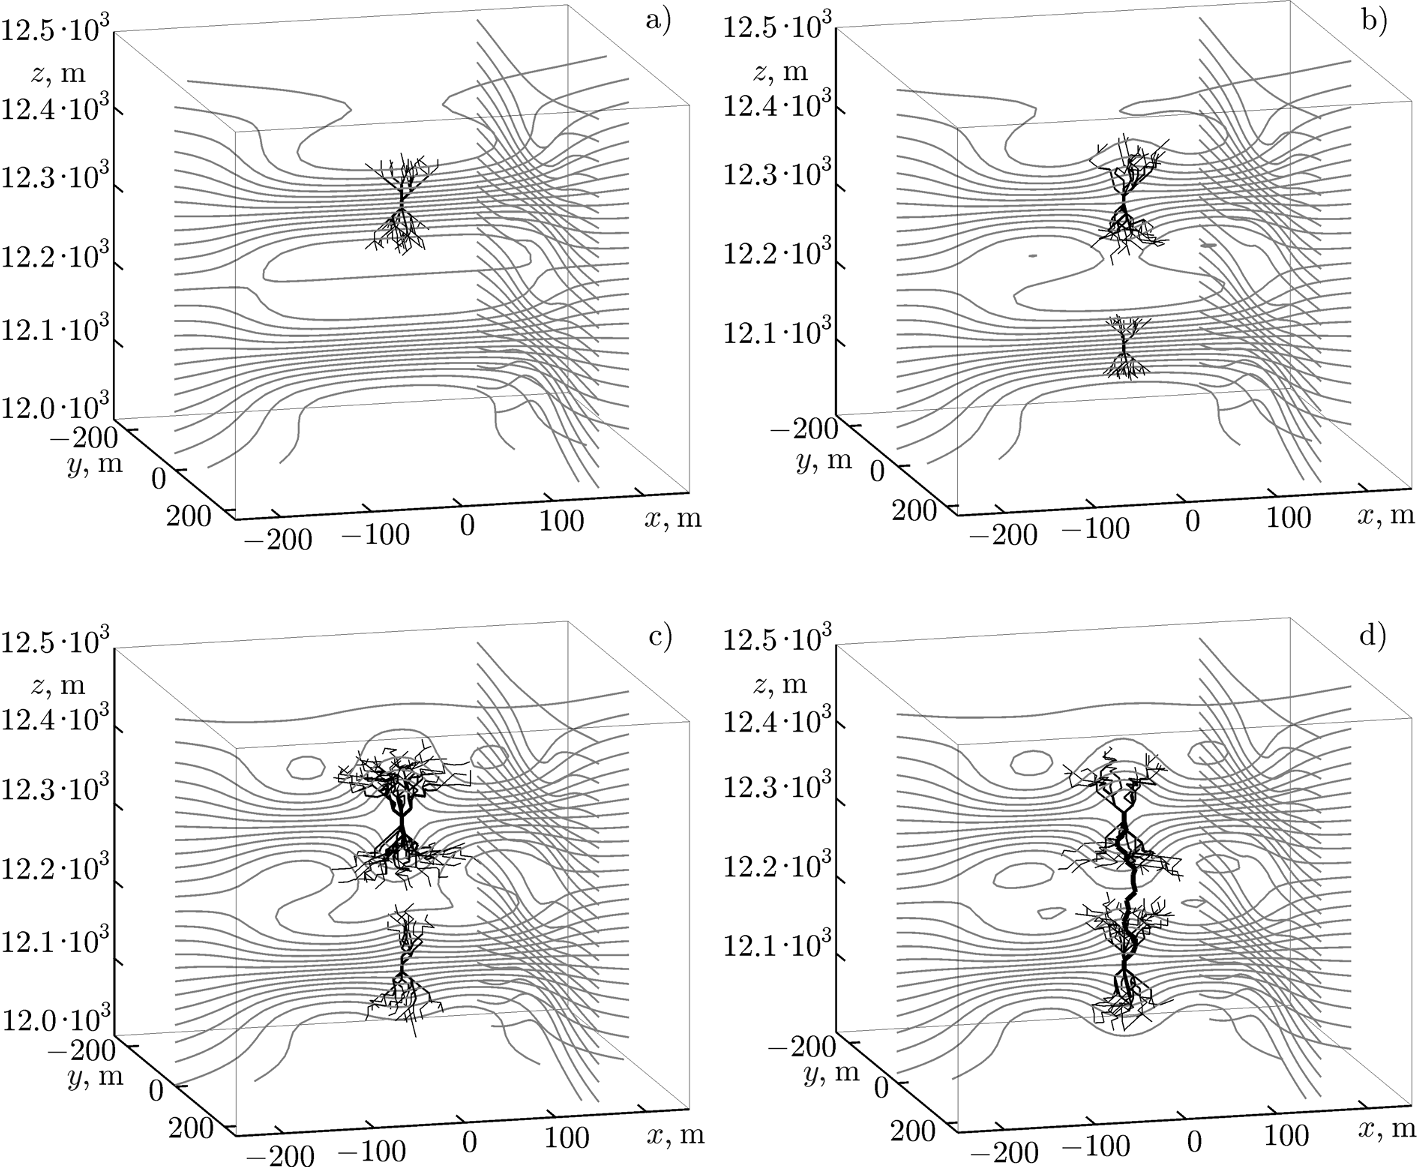
\includegraphics[width=0.9\textwidth]{imagens_artigo/14.png}
				\captionof{figure}{Desenvolvimento passo a passo de um \textit{CID}}
			\end{figure}
		\end{column}
		\begin{column}[c]{0.5\textwidth}
			Desenvolvimento passo a passo do \textit{CID}:
			\begin{enumerate}[(a)]
				\item Primeiro \textit{streamer} bipolar;
				\item Segundo \textit{streamer} bipolar;
				\item Desenvolvimento dos \textit{streamers} até atingirem o contato;
				\item Iniciação da Descarga Compacta Intra-Nuvem.
			\end{enumerate}

		\end{column}
	\end{columns}
\end{frame}

\begin{frame}{\textit{Resultados}}
	\begin{columns}
		\begin{column}{0.67\textwidth}
			\begin{figure}
				\centering
				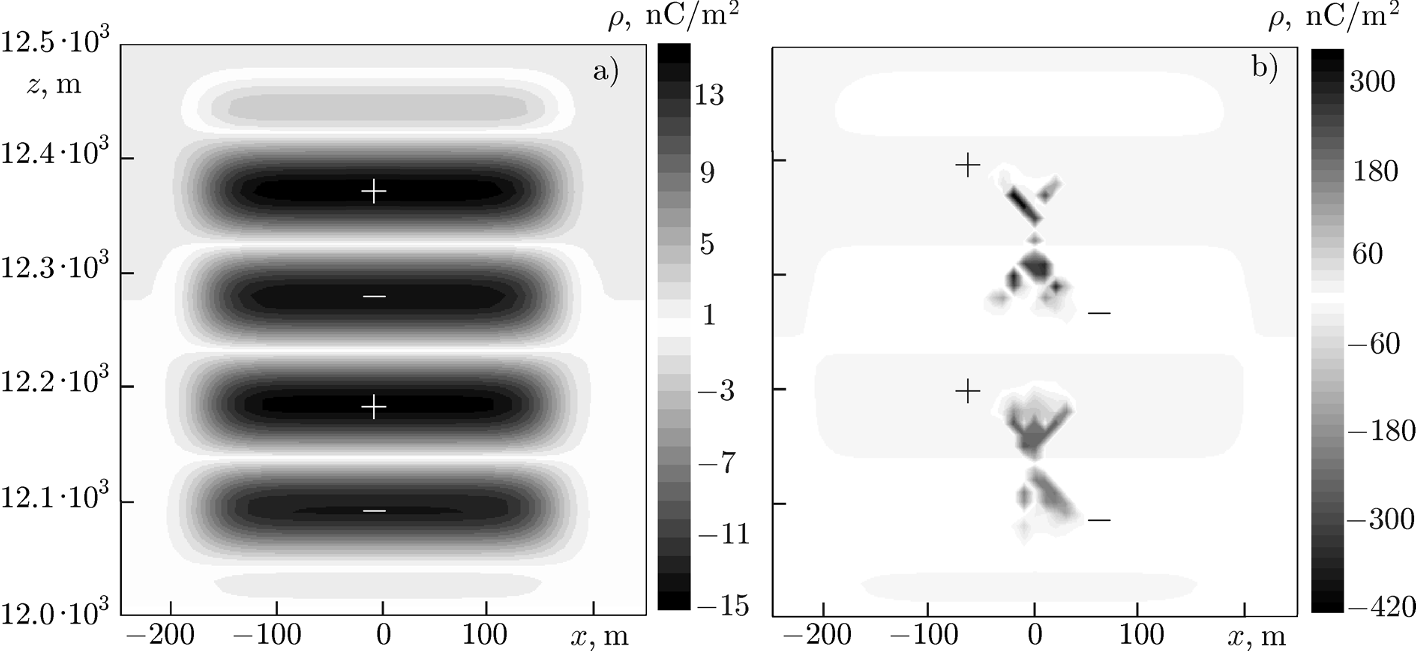
\includegraphics[width=0.9\textwidth]{imagens_artigo/15.png}
			\end{figure}
		\end{column}
		\begin{column}{0.33\textwidth}
			\begin{figure}
				\centering
				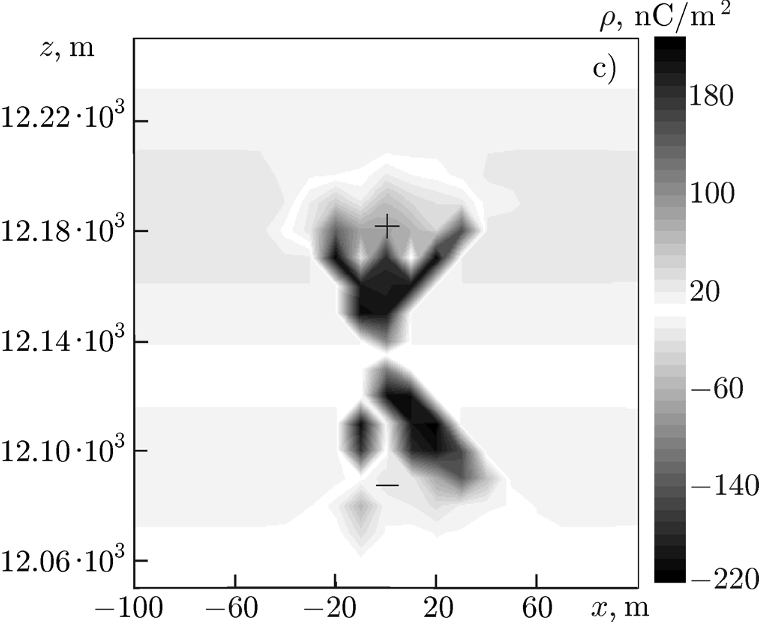
\includegraphics[width=\textwidth]{imagens_artigo/16.png}
			\end{figure}
		\end{column}
	\end{columns}
\end{frame}

\begin{frame}{\textit{Resultados}}

	\begin{figure}
		\centering
		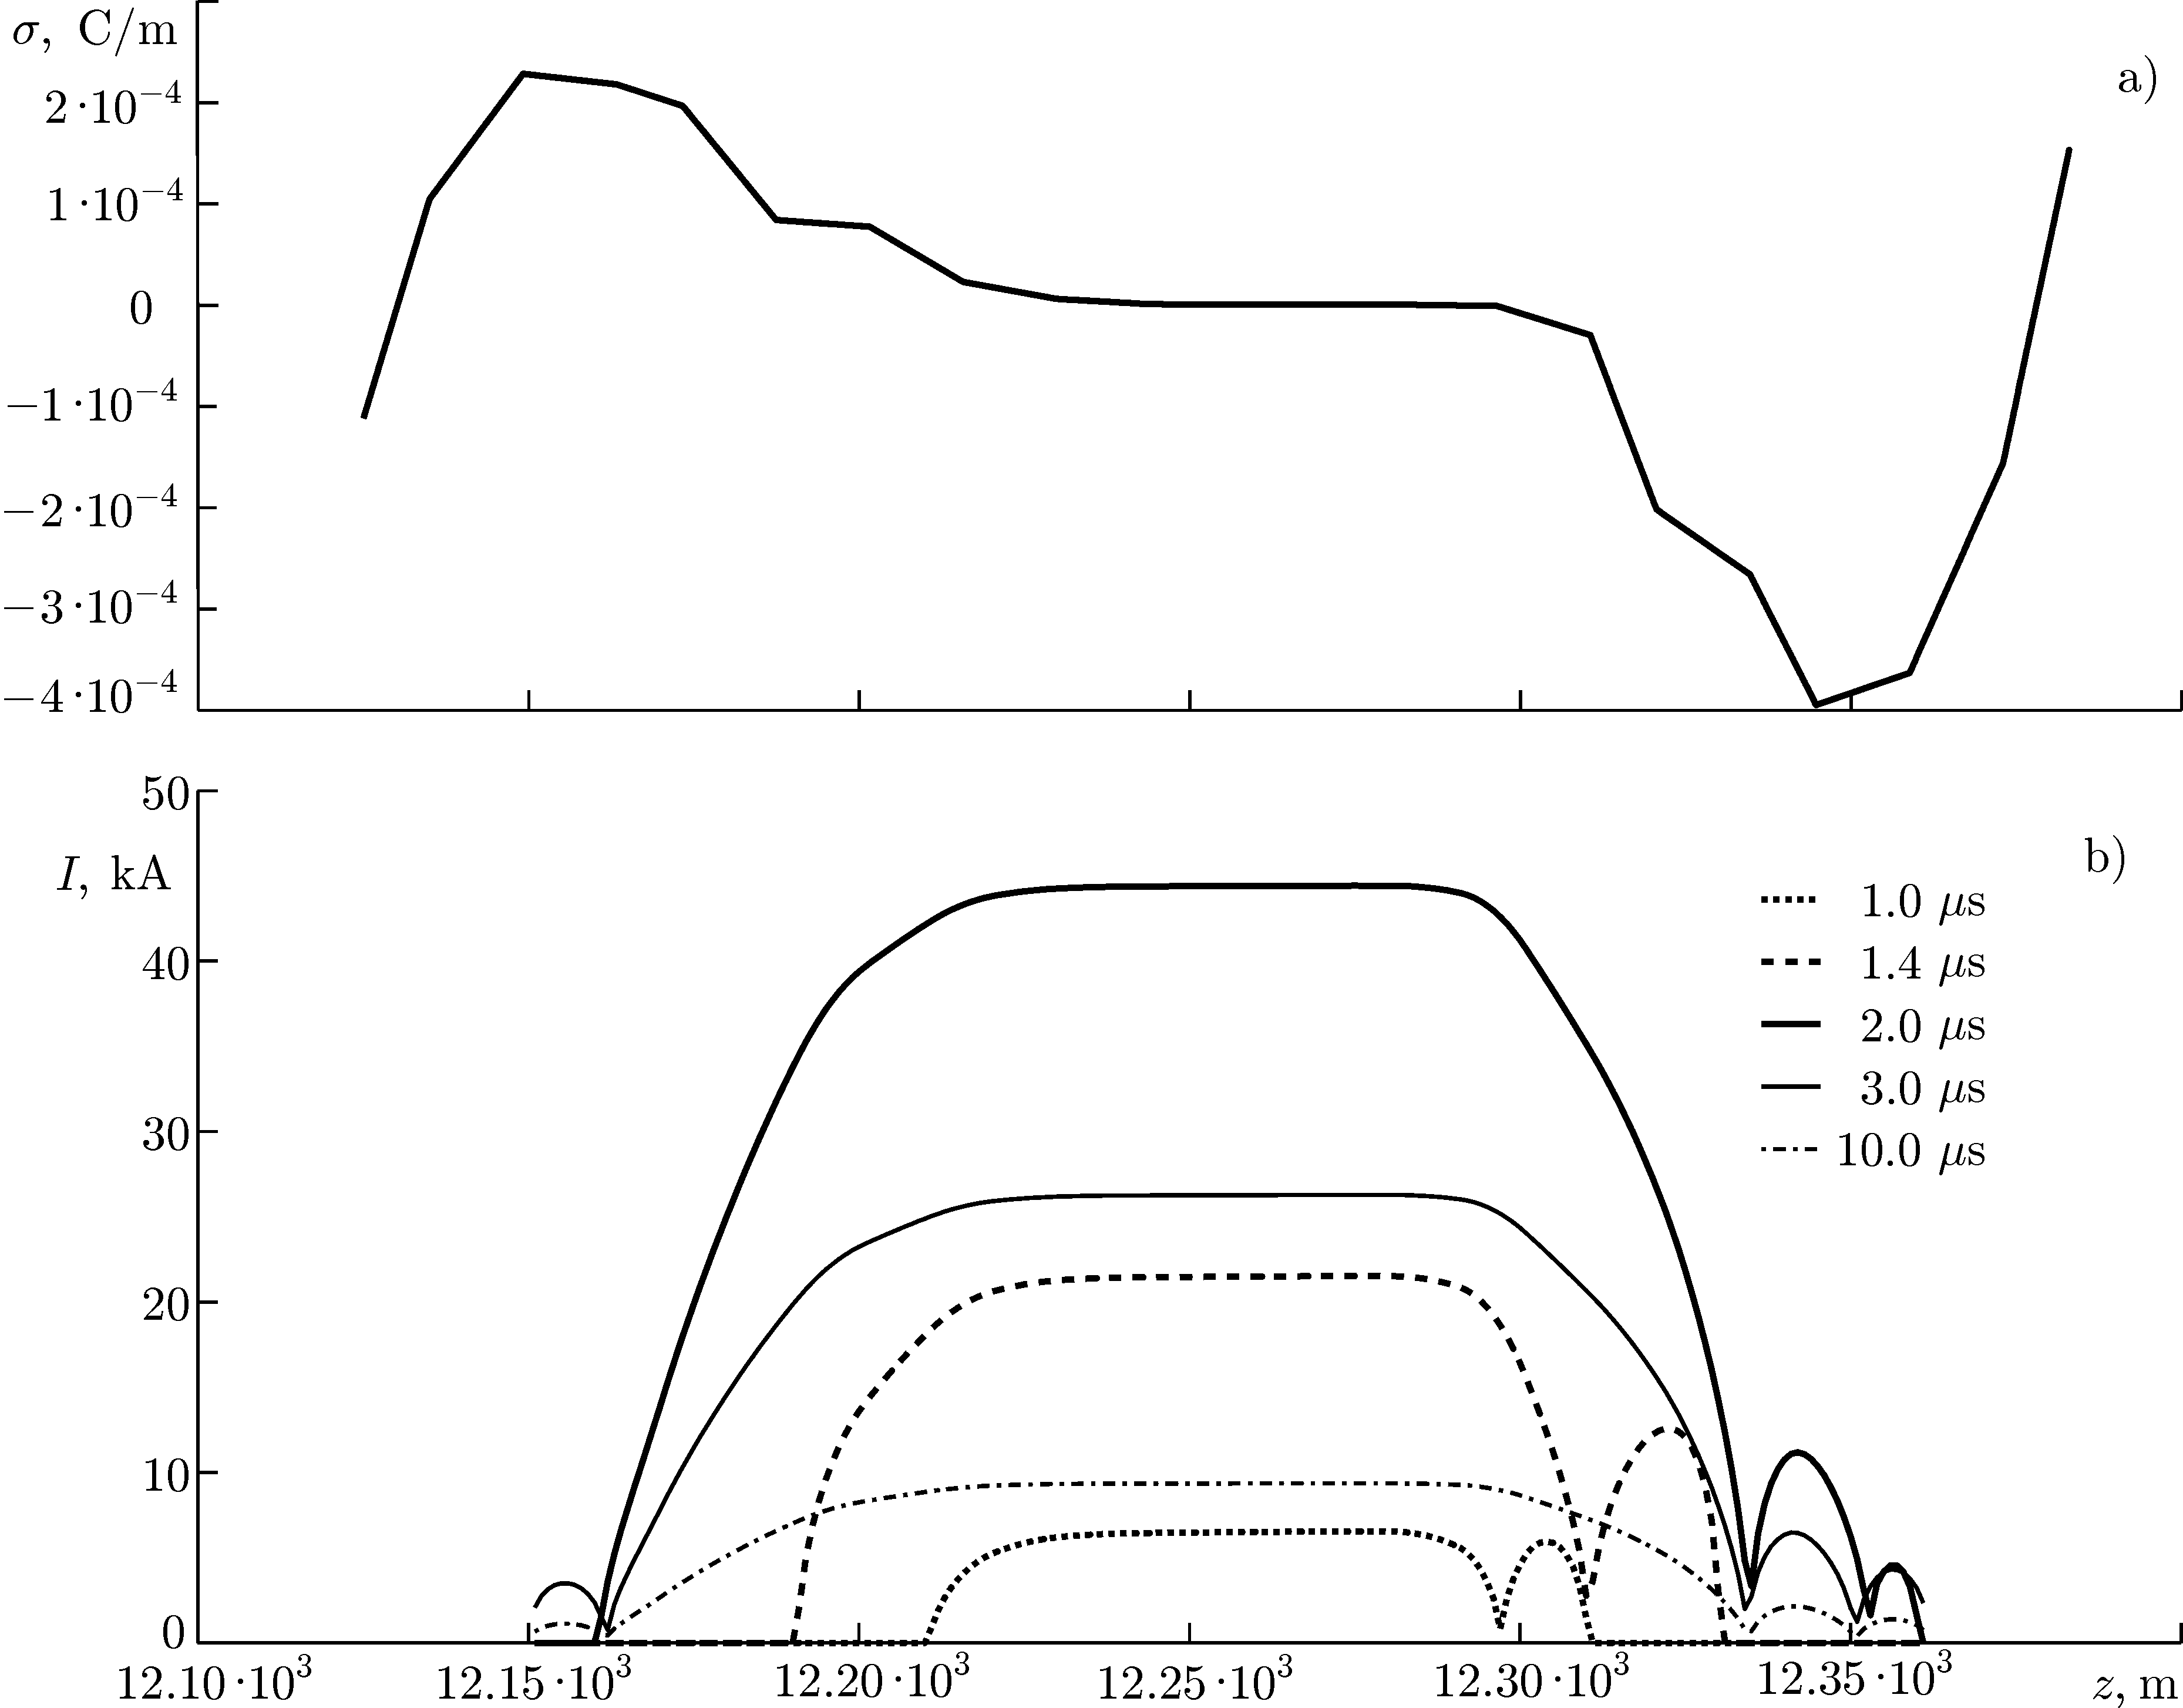
\includegraphics[width=0.45\textwidth]{imagens_artigo/17.png}
		\captionof{figure}{Densidade de Carga Linear e Corrente ao longo do Canal}
	\end{figure}

\end{frame}

\begin{chapter}[images/tema_fundo_3.png]{uicblue}{Conclusões}
\textit{Calma, já vamos embora}
\end{chapter}
\begin{frame}{\textit{Conclusões}}
	 Dentro da abordagem proposta, é possível explicar diversas características observadas da descarga compacta intra-nuvem, como a fraca radiação durante a etapa preliminar da descarga (abaixo dos limites de detecção estabelecidos nos experimentos), a formação de um curto pulso bipolar de campo elétrico de alta potência e a sincronização das rajadas de radiação nas faixas \textit{VLF/LF} e \textit{HF/VHF}. A radiação em diferentes faixas de frequência de uma descarga compacta intra-nuvem será abordada na segunda parte do trabalho.
\end{frame}
\backmatter
\end{document}
